%modeling

\section{persona}

\subsection{preparement}

After figured out the main problem it was time to use our fantasy. We should create a typical CARMEQ worker based on our results
of the interviews. This person is called 'persona'. In each phase of the development we will need him to help us to find our
target. It doesn't make sense to create a application in the intention to satisfy everybody, its better to shrink the requirements
to avoid to have in the end a program which can do a little bit of everything, where nobody knows what he can really do with. 

\subsection{implementation}

We started with 2 prototypes, one with the bahncard50 and the other with bahncard100. Finally we choosed the second because in our
opinion he has more problems on which we could have an influence. The typical CARMEQ worker is middle-aged, ambitious with a
high education level. In the reason of having the bahncard he has to travel a lot, the main reason for this is that he could work
as project manager.  We created a person named 'Batur Temel', the whole persona is shown in \prettyref{fig:persona1}, 
\prettyref{fig:persona2},  \prettyref{fig:persona3} and  \prettyref{fig:persona4}.

\clearpage

\begin{figure}[!h]
	\includegraphics[scale=0.8, page=1]{images/Persona_final.pdf}
	\caption{persona sheet 1}
	\label{fig:persona1}
\end{figure}

\clearpage

\begin{figure}[!h]
	\includegraphics[scale=0.8, page=2]{images/Persona_final.pdf}
	\caption{persona sheet 2}
	\label{fig:persona2}
\end{figure}

\clearpage

\begin{figure}[!h]
	\includegraphics[scale=0.8, trim=0mm 20mm 0mm 20mm,clip,page=3]{images/Persona_final.pdf}
	\caption{persona sheet 3}
	\label{fig:persona3}
\end{figure}

\begin{figure}[!h]
	\includegraphics[trim=0mm 240mm 0mm 20mm,clip,scale=0.8, page=4]{images/Persona_final.pdf}
	\caption{persona sheet 4}
	\label{fig:persona4}
\end{figure}

\section{point of view}

\subsection{preparement and  implementation}

The point of view helps also to clarify which requirements we want to handle. We tried to see with the eyes of our persona and
work them out. He has a problem with his payoff because of his bahncard100 usually he has no proof when he did a travel. In
addition he has also the problem with the seat reservation and the taxi-use.

\begin{figure}[!h]
	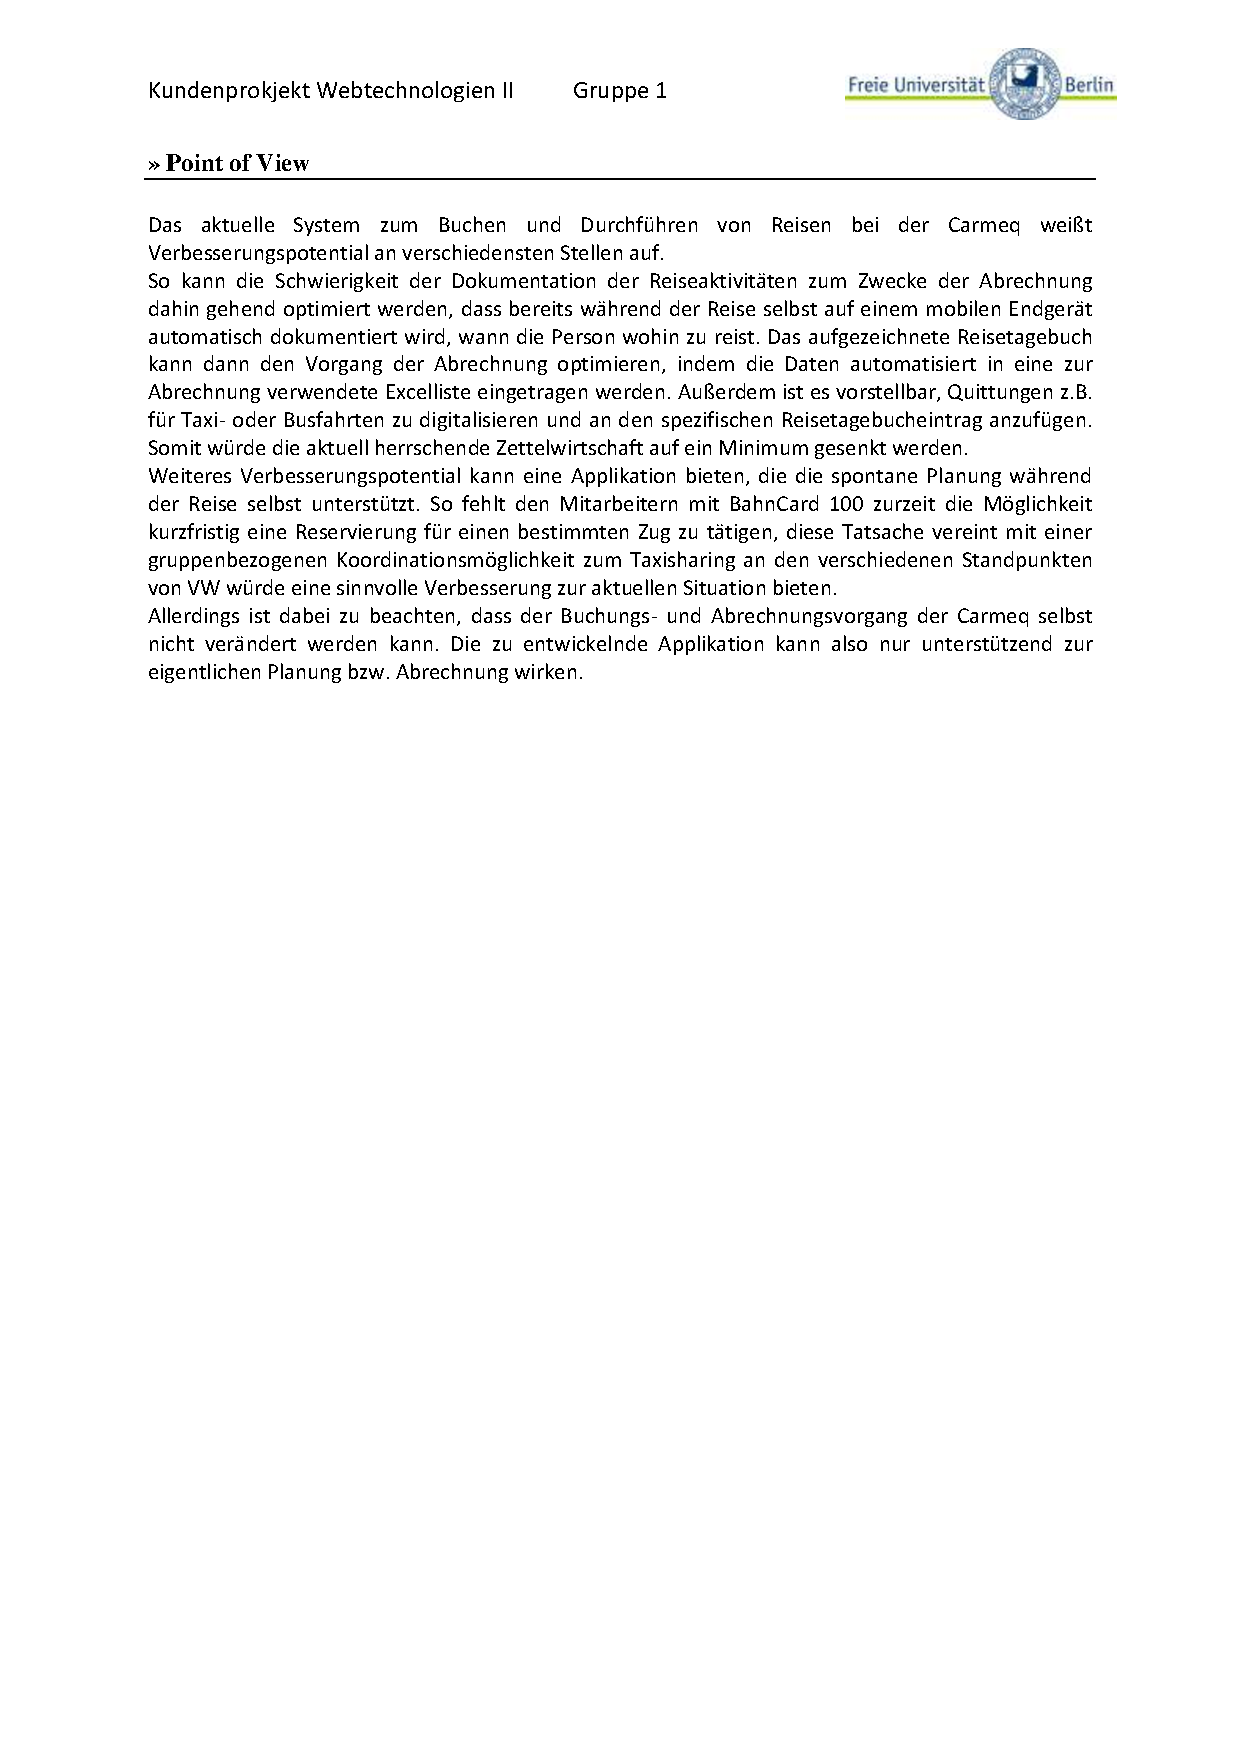
\includegraphics[trim=0mm 140mm 0mm 20mm,clip,scale=0.8, page=1]{images/POV.pdf}
	\caption{point of view}
	\label{fig:pov}
\end{figure}

\clearpage

